\chapter{Anhang}

\section{MRiLab auf "GPU-Rechner"}%%%%%%%%%%%%%%%%%%%%%%%%%%%%%%%%%%
\label{sec:usedPC}
MRiLab wird auf einem Personal Computer mit der, in \autoref{tab:gpuPc} angegebenen, Hardware- und Software-Ausstattung installiert.

\begin{table}[H]
	\centering
	\caption{Spezifikationen des verwendeten Rechners}
	\begin{tabular}{ll}
		\toprule
		\multicolumn{2}{c}{\textbf{Hardware}} \\
		CPU & Intel Xeon E5-1650v4 (3.6 GHz) \\
		GPU & Nvidia GeForce GTX Titan X \\
		RAM & 2x8 GB \\
		\midrule
		\multicolumn{2}{c}{\textbf{Software}} \\
		OS & Microsoft Windows 10 Pro for Workstations \\
		MATLAB & R2018a \\
		GPU Driver & Nvidia 398.82 \\
		CUDA & 7.0 \\
		\bottomrule
	\end{tabular}
	\label{tab:gpuPc}
\end{table}

Andere getestete Konfigurationen:
\begin{enumerate}
	\item \textbf{Ubuntu 18.04, CUDA 9.2}: CUDA 9.2 unterstützt offiziell nur Ubuntu 16.04 und 17.10. Die Installation von CUDA war dennoch erfolgreich\footnote{siehe https://devtalk\-.nvidia.com/\-default/topic/983777/\-cuda-setup-and-installation\-/can-t-locate-installutils\--pm-in-inc/}. 
	Die CUDA Libraries werden aber von \texttt{DoScanAtGPU} in MRiLab nicht gefunden (Von MRiLab wird versucht libcudart.so.7 statt allgemein libcudart.so zu laden).
	
	\item\label{en:versuch2} \textbf{Ubuntu 18.04, CUDA 7.0}: CUDA 7.0 unterstützt offiziell nur Ubuntu 14.04, 14.10 und 12.04. Die Installation ist dennoch ohne Probleme möglich. Die CUDA Libraries werden von MRiLab gefunden und ein Scan kann gestartet werden. Gegen Ende der Simulation stürzt MATLAB jedoch aufgrund eines Laufzeitfehlers in \texttt{DoScanAtGPU} ab.
	
	\item \textbf{Ubuntu 16.04, CUDA 7.0}: Fehlerbild wie unter Punkt \ref{en:versuch2}.
	
	\item \textbf{Ubuntu 14.04, CUDA 7.0}: MATLAB bzw. MRiLAB aufgrund eines Bugs nicht benutzbar ("dlopen: cannot load any more object with static TLS")
	
\end{enumerate}

\section{Modifikationen MRiLab GUI}%%%%%%%%%%%%%%%%%%%%%%%%%%%%%%%%%
Für die, in dieser Arbeit vorgenommenen, Erweiterungen von MRiLab ist es von Vorteil, Simulationsparameter unkompliziert über die GUI anpassen zu können. Dazu müssen die gewünschten Bedienelemente in die bestehende GUI eingefügt werden.

\subsection{Struktur der MRiLab GUI}
MRiLab besteht aus einem Hauptfenster (\texttt{SimuPanel}) und mehreren Zusatzfenstern, den sog. "Design Panels". Das Haupt- und die Zusatzfenster sind jeweils mit dem MATLAB GUI Layout Editor \textit{GUIDE} (GUI development environment) erzeugt worden.

Ein GUIDE Fenster besteht aus zwei Dateien: Die .fig Binärdatei kann nur mit GUIDE geöffnet werden und enthält eine Beschreibung des Layouts. GUIDE erzeugt aus dieser eine MATLAB .m-Datei. Diese enthält Coderümpfe, um auf die im Layout spezifizierten Elemente zuzugreifen.

\subsubsection{Einbau eines neuen GUI Elements}
Zum Einbau eines neuen GUI Elements in das MRiLab Hauptfenster wird GUIDE aus MATLAB heraus gestartet (\texttt{>>guide}) und die Datei \texttt{SimuPanel.fig} geöffnet. Nach dem Einfügen eines neuen Elements wird die Datei gespeichert. Die Datei \texttt{SimuPanel.m} wird dadurch im MATLAB Editor geöffnet und die "create"- bzw. "callback"-Funktion werden automatisch generiert.

\subsubsection{Zugriff auf neue GUI Elemente}
GUIDE benutzt die Variable \texttt{handles}, um Daten zwischen GUI Elementen auszutauschen. Die Variable handles besteht aus einem Struct und kann auch für Benutzer-definierte globale Variablen benutzt werden. Dadurch ist der Zugriff aus allen GUI Teilen einfach möglich.

Auch, wenn die Programmierung mit globalen Variablen einige Probleme mit sich bringt\footnote{Programmteile schwierig isoliert zu testen, Auftreten von Namenskonflikten, etc.}, wird die oben erläuterte Vorgehensweise dennoch verwendet, um konsistent mit dem bestehenden Code zu sein.

Um aus einem Submodul (ohne GUI) auf ein Element des handles Struct zugreifen zu können, wird der Struct normal als Funktionsparameter übergeben.

\subsubsection{Beispiel}
Mit GUIDE wird ein Textfeld "phaseNoiseLevel" in das Hauptfenster eingebaut.
Auf den Wert in dem Textfeld soll aus \texttt{DoAddNoise.m} zugegriffen werden. \texttt{DoAddNoise.m} wird über \texttt{DoPostScan.m} von \texttt{SimuPanel.m} aufgerufen. Der handles Struct wird im Original MRiLab DoPostScan.m übergeben. Es muss daher lediglich der Parameterliste von \texttt{DoAddNoise.m} hinzugefügt werden.

\begin{listing}[H]
	\begin{minted}[bgcolor=bg,fontsize=\footnotesize,linenos,autogobble]
	{Matlab}
	function DoAddNoise(handles)
	% Add noise in K-space data
	
	global VSig;
	global VCtl;
	
	uiPhaseNoiseLevel=str2num(get(handles.phaseNoiseLevel,'String'));
	...
	\end{minted}
	\caption{Beginn der Funktion \texttt{DoAddNoise.m} mit Zugriff auf \texttt{handles.phaseNoiseLevel}}
	\label{lst:doAddNoisesimuh}
\end{listing}

Ist die Definition von \texttt{DoAddNoise.m} um das "handles" Struct erweitert (siehe \autoref{lst:doAddNoisesimuh}), kann der Funktion das Struct von \texttt{DoPostScan.m} übergeben werden (\autoref{lst:doPostscansimuh}, Zeile 10).


\begin{listing}[H]
	\begin{minted}[bgcolor=bg,fontsize=\footnotesize,linenos,autogobble]
	{Matlab}
	function DoPostScan(Simuh)
	
	global VCtl
	global VImg
	global VCoi
	DoUpdateInfo(Simuh,'Scan is complete!');
	set(Simuh.TimeWait_text,'String', ['Est. Time Left :  ' '~' ' : ' '~' ' : ' '~']);
	%% Signal Post-Processing
	%  Add noise
	DoAddNoise(Simuh);
	...
	\end{minted}
	\caption{Funktion \texttt{DoPostScan.m} übergibt "handles" Struct (mit Name "Simuh") an \texttt{DoAddNoise.m}}
	\label{lst:doPostscansimuh}
\end{listing}

\section{Kommerzielle MRT-Phantome}

\begin{table}[H]
	\caption{Auswahl einiger am Markt verfügbarer MRT Phantome (Stand August 2018)}
	\centering
	\begin{tabularx}{\textwidth}{l X l}
		\toprule
		\textbf{Abbildung} & \textbf{Beschreibung} & \textbf{günstigstes Angebot} \\
		\midrule \\[5pt]
		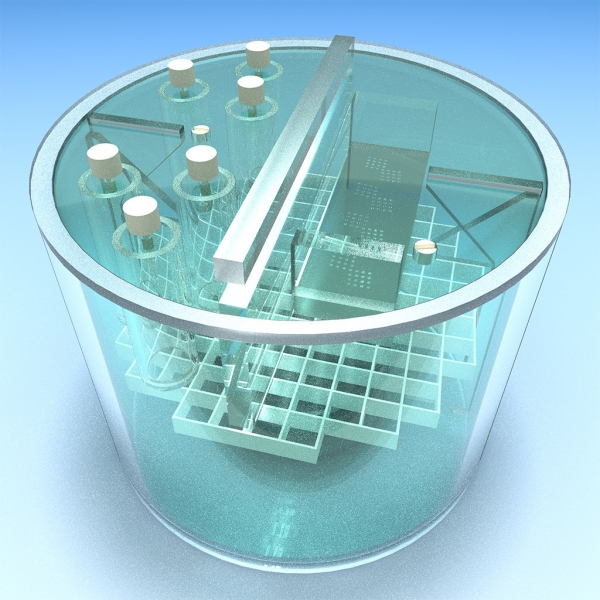
\includegraphics[width=0.25\textwidth,valign=t]{img/phantoms/allMRI.jpg} & \textbf{allMRI/\-Pro-MRI \newline180mm phantom} \newline Außendurchmesser: \SI{180}{\mm},\newline Höhe: \SI{150}{\mm} \newline \cite{allMRIphantom} & 1235€ \\
		&&\\
		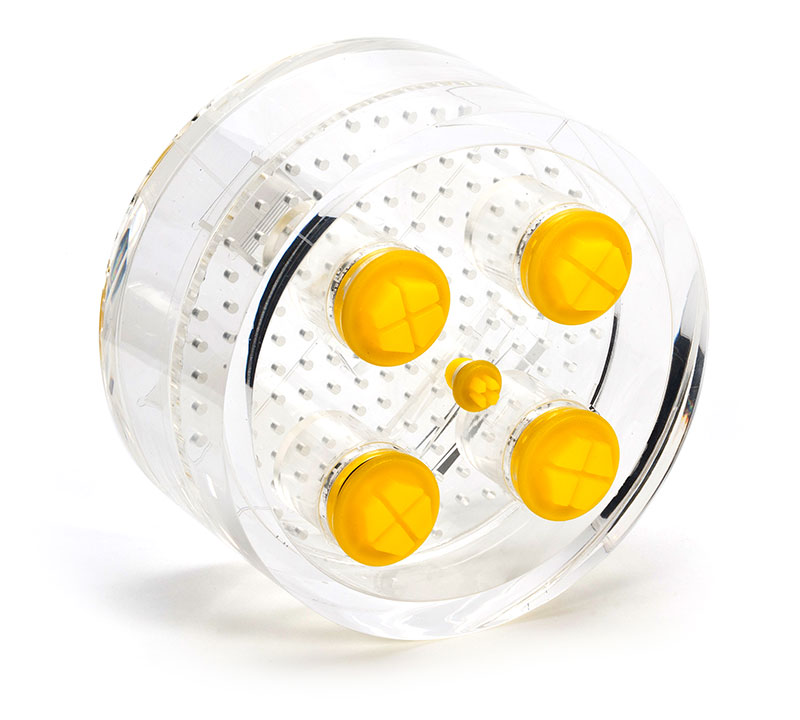
\includegraphics[width=0.25\textwidth,valign=t]{img/phantoms/MagIQ.jpg} & \textbf{Leeds MagIQ 142} \newline Außendurchmesser: \SI{142}{\mm},\newline Höhe: \SI{70}{\mm} \newline \cite{leeds} & 3250€ \\
		&&\\
		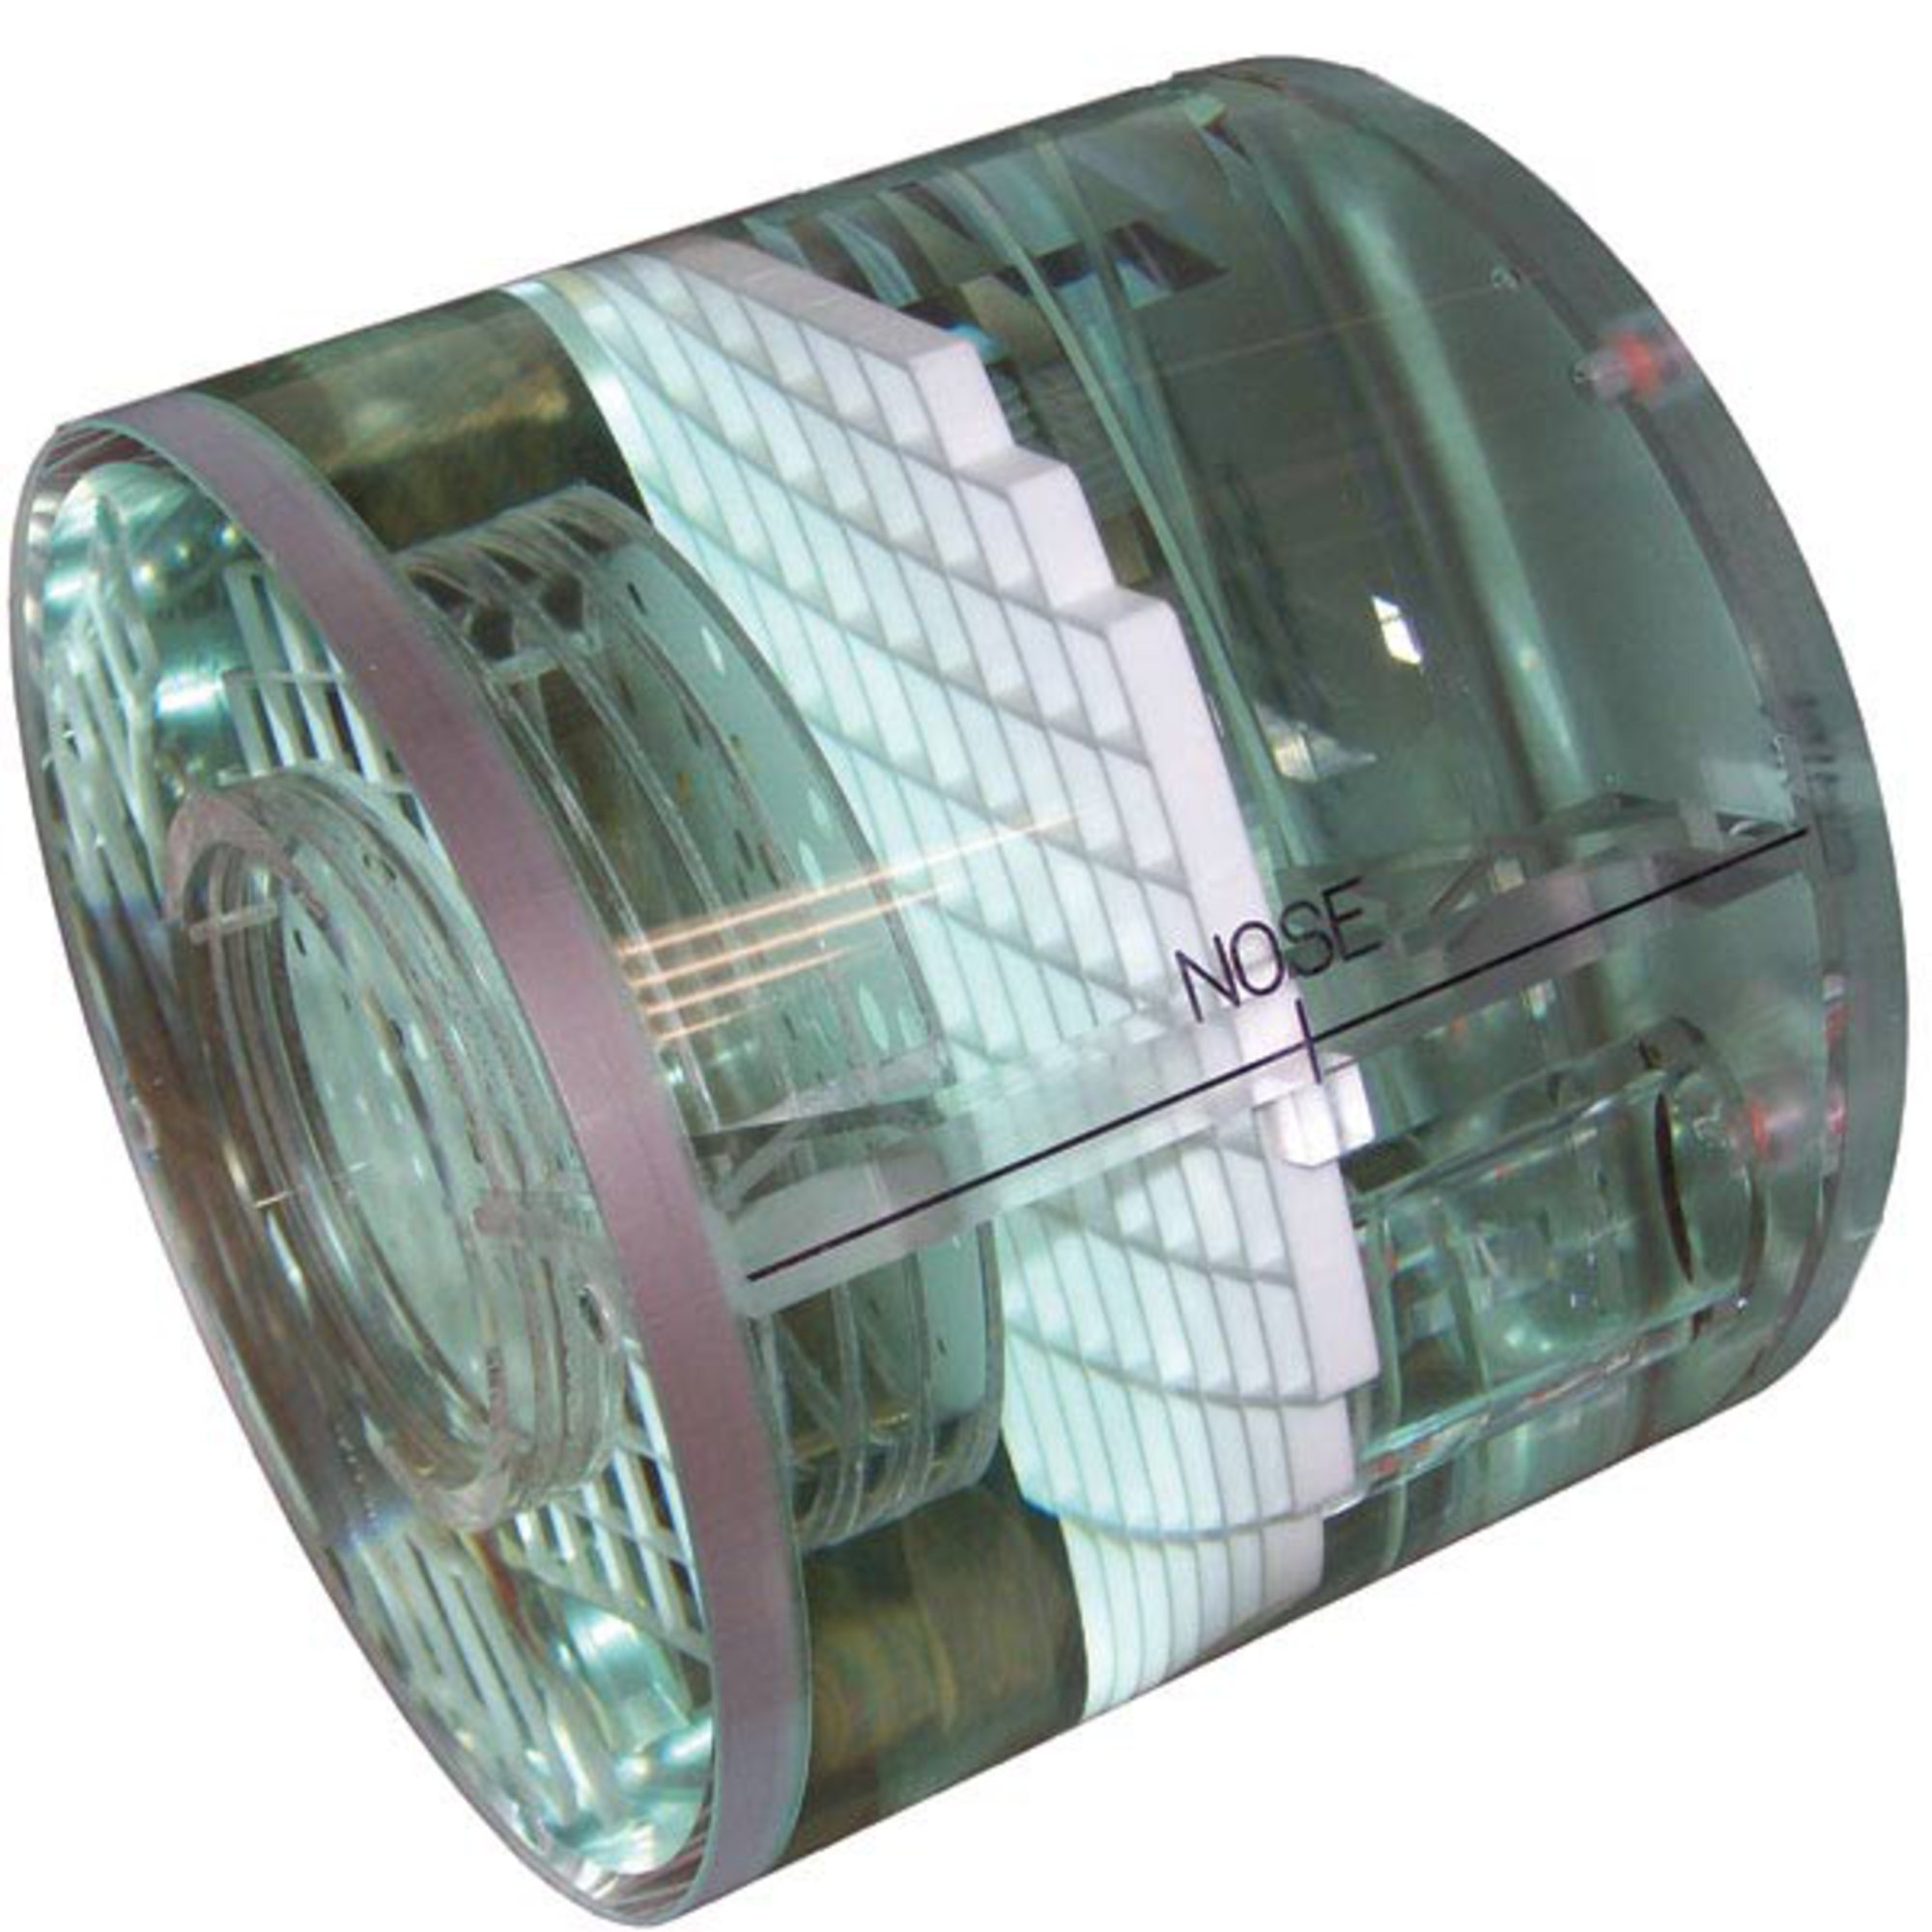
\includegraphics[width=0.25\textwidth,valign=t]{img/phantoms/acr.jpg} & \textbf{ACR MRI Phantom} \newline Außendurchmesser: \SI{203}{\mm},\newline Höhe: \SI{173.4}{\mm} \newline \cite{acr}  & 1800€ \\
		&&\\
		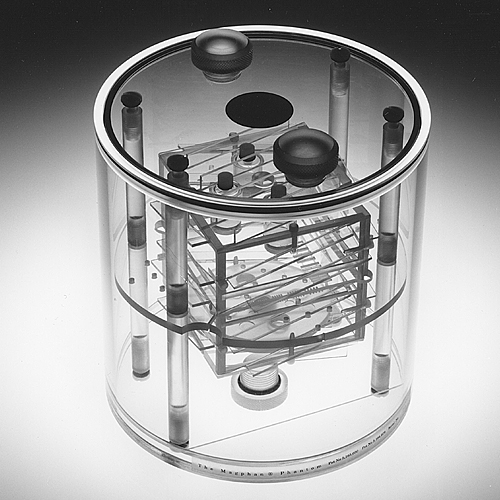
\includegraphics[width=0.25\textwidth,valign=t]{img/phantoms/Magphan.jpg} & \textbf{MAGPHAN CYLINDRICAL 170} \newline Außendurchmesser: \SI{200}{\mm} \newline \cite{mag170}  & - \\
		&&\\
		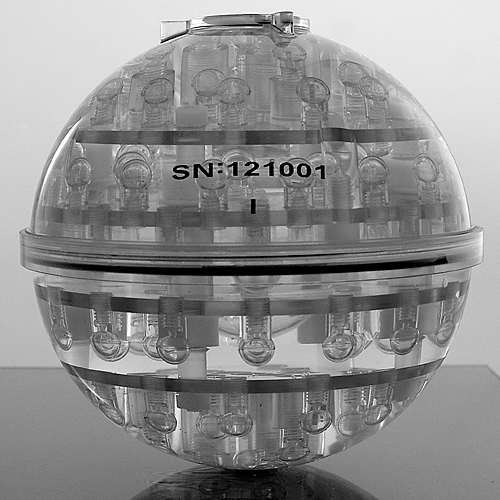
\includegraphics[width=0.25\textwidth,valign=t]{img/phantoms/magphan121.jpg} & \textbf{MAGPHAN MR Distortion Phantom (ADNI) 121} \newline Außendurchmesser: \SI{200}{\mm} \newline \cite{mag121} & - \\
		&&\\
		\bottomrule
		\end{tabularx}
		\label{tab:phantomsOverview}
		\end{table}
